% -*- mode: fundamental -*-

% ****************************************************************

\chapter{BSV: Rules and their Semantics}

\markboth{Ch \arabic{chapter}: BSV: Rules I}{\copyrightnotice}

\setcounter{page}{1}
% \renewcommand{\thepage}{\arabic{page}}
\renewcommand{\thepage}{\arabic{chapter}-\arabic{page}}

\label{ch_Rules_I}

% ****************************************************************

\section{Introduction}

``\emph{Rules}'' are the fundamental constructs in BSV to specify
dynamic behavior.  Rules appear in the body of BSV modules, and they
may invoke methods in interfaces of other modules.  An interface
method is simply a ``mini-rule'' that is incorporated into a rule from
which it is invoked.  Rule semantics can be understood in two
incremental steps:

\begin{tightlist}

 \item Semantics of a rule in isolation (Section~\ref{Sec_Single_Rule_Semantics})

 \item Semantics of the collection of rules in a BSV program
       (Section~\ref{Sec_Rules_Semantics})

\end{tightlist}

Finally, the performance of rules (how long does a computation take?)
can be understood by understanding how rules are mapped to a clock
(Section~\ref{Sec_Mapping_Rules_to_a_Clock})

% ****************************************************************

\section{Syntax of a rule and the data types of its components}

\index[BSV]{Rules!Syntax and types}


Figure~\ref{Fig_Rule_Structure} shows the syntactic structure of a
rule, with the keywords \verb|rule| and \verb|endrule|.
\begin{figure}[htbp]
  \centerline{\includegraphics[width=6in,angle=0]{Figures/Fig_Rule_Structure}}
  \caption{\label{Fig_Rule_Structure} Syntactic structure of a rule}
\end{figure}

\index[BSV]{Rules!Explicit condition}

The rule's \emph{explicit} condition is an expression of type
\verb|Bool|.  Recall from
Section~\ref{Sec_Pure_vs_Side_Effect_functions} that, since it is not
of \verb|Action| or \verb|ActionValue| type, it is guaranteed by BSV's
type system therefore to be a pure computation with no side-effects.

\index[BSV]{Rules!Body, of type {\tt Action}}

The rule body, as a whole, is an expression of type \verb|Action|.  It
typically consists of multiple statements, including register-writes,
FIFO enqueues/dequeues, module method invocations,
\verb|let|-bindings, \verb|$display|s, if-then-elses|, and so on.
Many of the statements/sub-expressions will themselves be of type
\verb|Action| or \verb|ActionValue|.  The overall action of a rule is
the set of all sub-actions performed by a rule.

\index[BSV]{Rules!Implicit/READY condition}

Both the rule condition and the body may contain invocations of
methods in interfaces of other modules.  Each method has an ``implicit
condition'', also of type \verb|Bool| indicating whether the method is
currently enabled or not.  This implicit method output is also called
its READY signal.  For example, for a standard FIFO $f$, the
$f$\verb|.first| and $f$\verb|.deq()| methods have implicit conditions
that are true only when the FIFO is non-empty.  A method like
$f$\verb|.first|, being pure (not \verb|Action| or
\verb|ActionValue|), may be invoked both in rule conditions and in
rule bodies.  A method like $f$\verb|.deq|, being of type
\verb|Action|, can never be invoked in a rule condition, only in a
rule body.

The overall rule condition, also known as its ``CAN\_FIRE'' condition,
is a conjunction of the rule's explicit condition and implicit
conditions of any invoked methods (whether those methods are in the
rule condition or in the rule body).  For example, if a rule invokes
$f$\verb|.first| or $f$\verb|.deq|, the rule's CAN\_FIRE condition
cannot be true if $f$ is empty.

% ****************************************************************

\section{Semantics of a rule in isolation}

\label{Sec_Single_Rule_Semantics}

\index[BSV]{Rules!Semantics of individual rule}

In this section we discuss the semantics of a rule in isolation; in
Section~\ref{Sec_Rules_Semantics} we will consider the collection of
rules that constitute a BSV design.

Each rule can be viewed as a pure function (therefore, a combinational
circuit) whose inputs come from various methods and which produces
outputs for various \verb|Action| and \verb|ActionValue| methods.
Each \verb|Action| or \verb|ActionValue| method has an implicit
boolean ENABLE argument (separate from its normal arguments and
result).  An \verb|Action| or \verb|ActionValue| method
\emph{performs} its action if its ENABLE argument is true.

Consider the following rule (artificial, just for illustration, not
taken from code of Drum or Fife or any actual design):

{\small
\begin{Verbatim}[frame=single, numbers=left]
   rule rl_compute ((y != 0) && got_x && (f.first == 3));
    if (y [0] == 1) w <= w + x;
    x <= x << 1;
    g.enq (w * f.first);
   endrule
\end{Verbatim}
}

Figure~\ref{Fig_Rule_Actions_1} illustrates the semantics of this rule
in isolation.
\begin{figure}[htbp]
  \centerline{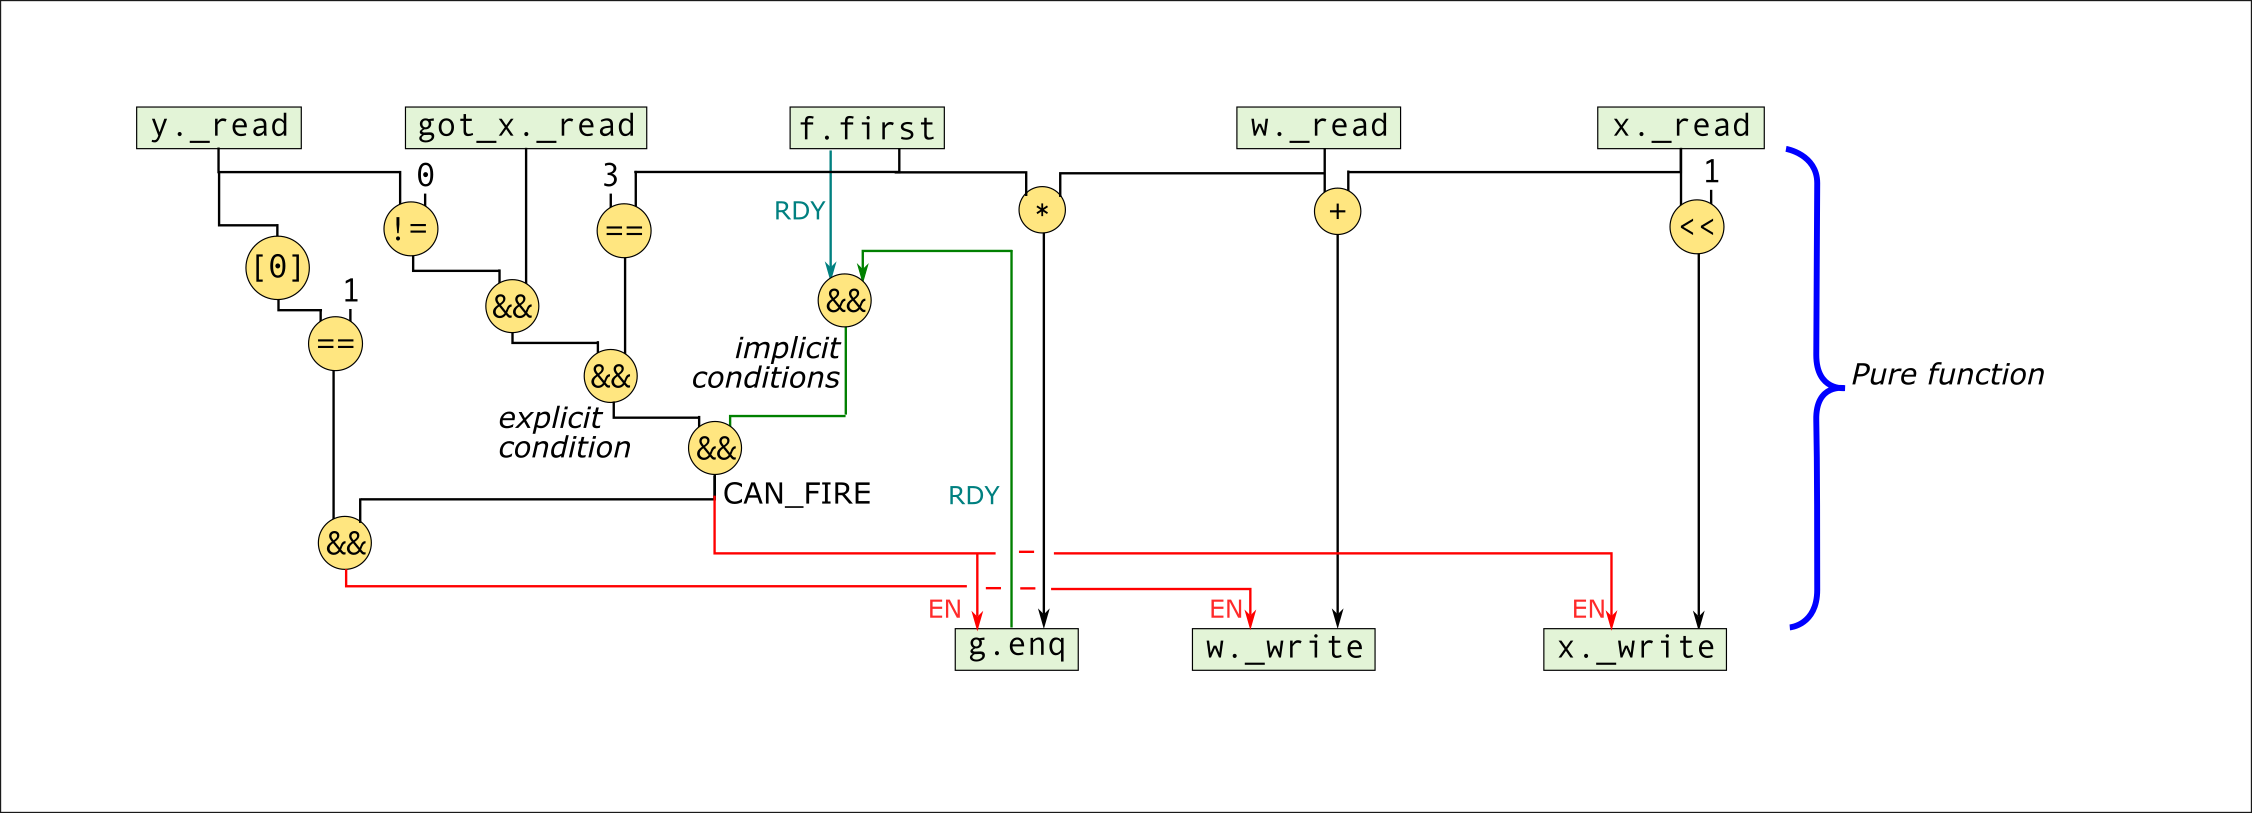
\includegraphics[width=6in,angle=0]{Figures/Fig_Rule_Actions_1}}
  \caption{\label{Fig_Rule_Actions_1} Semantics of a rule in isolation}
\end{figure}
In the discussion below, we use the words ``input'' and ``output''
relative to a method (input to the method, or output from the method).

At the top of the diagram we see outputs from methods feeding the
rule: four register-reads\footnote{Recall from
Section~\ref{Sec_Register_interface} mentioning a register in an
expression is equivalent to using its {\tt .\_read} method, and
assigning a value to a register is equivalent to using its {\tt
.\_write} method.} and one FIFO \verb|.first|.  The latter provides
two outputs: a data output from the head of the FIFO (black line) and
a READY value (green line) which is the implicit condition of the
method, which is true only if the FIFO is not empty.  Actually
\emph{all} methods have implicit conditions, but a register's
\verb|.read| and \verb|.write| methods are always READY, {\ie} their
implicit conditions are constant true, so we omit them in diagrams.

At the bottom of the diagram we see three \verb|Action| methods used
in the rule: two register-writes and one FIFO \verb|.enq|.  Each
method has an input data value (black line) and an implicit input
ENABLE value (red line).  The FIFO \verb|.enq| method also has a READY
output (green line), which is its implicit condition (true only when
the FIFO is not full).

In between the top and the bottom is a pure function (therefore, a
combinational circuit).  On the left half we see that all the
explicit-condition expressions are calculated and combined (with
``\verb|&&|''), and then further combined with the implicit
conditions, to produce the CAN\_FIRE signal.  This is fed directly to
the \verb|g.enq| and \verb|x._write| ENABLE inputs The CAN\_FIRE
signal is further combined with the calculation of ``\verb|y[0]==1|''
and this is fed to the ENABLE input of \verb|w._write|

The data inputs to the three \verb|Action| methods are straightforward
calculations from inputs.

When the ENABLE input to an \verb|Action| method is true, the method
actually performs the action (enqueue into a FIFO, store into a
register).

From the diagram we can see that the ENABLEs of \verb|g.enq| and
\verb|x._write| are true when FIFO \verb|f| has data available (not
empty), when FIFO \verb|g| has space available (not full) and when the
explicit condition is true---the rule ``fires'' and the actions are
performed.  The ENABLE of \verb|w._write| is true only if
\verb|y[0]==1| is also true.

From this description, several things should be clear:

\begin{itemize}

 \item All \verb|Action|s in a rule are performed
       \emph{simultaneously}, no matter what textual order they may
       appear in the rule body.  We also say that the actions all
       occur \emph{in parallel}.

 \item All \verb|Action|s in a rule are performed
       \emph{instantaneously}.

 \item Explicit rule conditions and method implicit conditions are
       combined to determine whether the rule executes at all.

 \item Some actions in a rule may be further restricted by
       if-then-else conditions in the rule.

\end{itemize}

% ================================================================

\subsection{Hardware representation of a rule in isolation}

\label{Sec_HW_representation_of_a_rule}

Figure~\ref{Fig_Rule_Actions_1_2} overlays standard symbols in digital
hardware for registers and FIFOs onto Figure~\ref{Fig_Rule_Actions_1},
to show how the semantics can map to real hardware in a
straightforward way.
\begin{figure}[htbp]
  \centerline{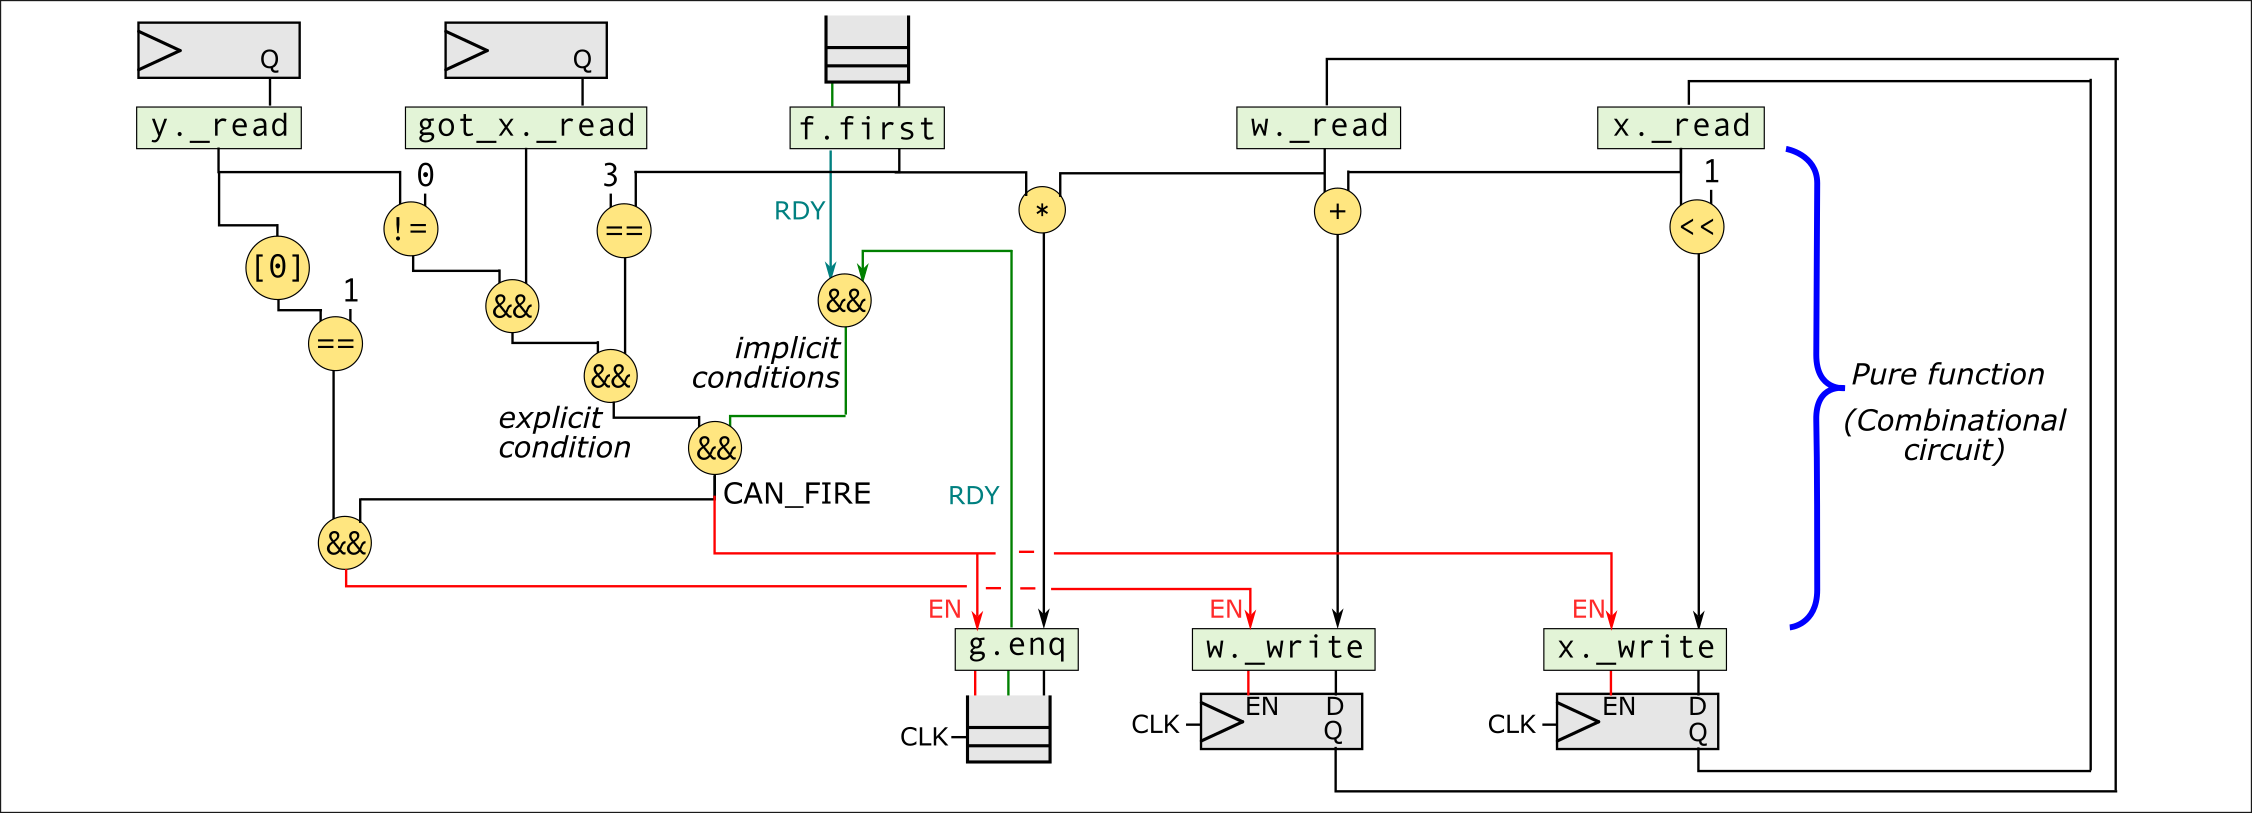
\includegraphics[width=6in,angle=0]{Figures/Fig_Rule_Actions_1_2}}
  \caption{\label{Fig_Rule_Actions_1_2} Hardware representation of a rule in isolation}
\end{figure}

BSV registers map directly into Verilog registers which, in turn, map
into ``D flip flops''.  The \verb|.read| method output is the same as
the ``Q'' outputs of D flip flops.  The \verb|.write| method inputs
are the same as the ``D'' and ``EN'' inputs of D flip flops.  Each
register also has a ``clock'' (CLK) input.  On each edge of CLK ({\eg}
on the positive edge, or so-called ``posedge'', when going from low to
high), if EN is true, then the value on the D input is copied into the
register, replacing the previous value.  The value in the register is
continuosly presented on the Q output wires.

BSV FIFOs are implemented as Verilog modules using registers.  The
details need not concern us here\footnote{If you are curious, you can
look at the FIFO Verilog codes in the \emph{bsc} library.} but,
suffice it to say, on a clock edge, if EN is true, the data value is
loaded into a register in the FIFO representing the tail of the queue.

In the semantics, we said that all actions of the rule are
``simultaneous''.  In hardware terms: they occur on the same clock
edge.

In the semantics, we said that all actions are ``instantaneous''.  In
hardware terms this is the standard digital abstraction, as if clock
edges are instantaneous, and as if registers load their values at that
instant.  In practice, because of physics, clock edges are steep but
not vertical (they have a small but finite rise times), but standard
digital abstraction suppresses this detail.

Standard digital abstraction also treats combinational circuits as
instantaneous, as if there is zero delay in producing outputs from
inputs.  In practice, signals take small but finite time to propagate
through wires and gates. Thus, the ENABLE for \verb|w._write| will be
available slightly later than the ENABLE for the other two methods,
because it goes through a longer combinational path.  But in the
standard digital abstraction we idealize all this as zero delay.

% ----------------
\vspace{2ex}

NOTE: \fbox{\small
\begin{minipage}{5in}

Although Figure~\ref{Fig_Rule_Actions_1_2} is useful in developing
intuitions, it is important to understand that BSV semantics stands
alone, and does not depend on any particular mapping to hardware!
Different compilers may map BSV to hardware in different ways, for
example using multiple clocks for some or all rules.  Indeed a
compiler could choose to map BSV code into so-called
``\emph{asynchronous logic}'' (which does not have clocks at all).

\end{minipage}}

\vspace{2ex}
% ----------------

% ----------------
\hdivider

\Exercise

Consider the following two alternative ways of writing a rule (that
differ only in the order of the rule-body statements):

\begin{center}
\begin{minipage}{2.5in}
 {\small
 \begin{Verbatim}[frame=single, label=BSV]
   rule rl_r1 (... condition ...);
    x <= y + 1;
    y <= x + 2;
   endrule
 \end{Verbatim}
 }
\end{minipage}
\hmm
\begin{minipage}{2.5in}
 {\small
 \begin{Verbatim}[frame=single,label=BSV]
   rule rl_r2 (... condition ...);
    y <= x + 2;
    x <= y + 1;
   endrule
 \end{Verbatim}
 }
\end{minipage}
\end{center}

\vspace{1ex}

Sketch the semantic view (and possible hardware) for the two
alternatives.  Is there any semantic difference between the two rules?

\vspace{1ex}

If the values of registers \verb|x| and \verb|y| are 10 and 20
respectively, what are their values after the rule fires once?  What
would the answer(s) be with the following similar-looking C
statements?

\begin{center}
\begin{minipage}{2.5in}
 {\small
 \begin{Verbatim}[frame=single, label=C]
    x = y + 1;
    y = x + 2;
 \end{Verbatim}
 }
\end{minipage}
\hmm
\begin{minipage}{2.5in}
 {\small
 \begin{Verbatim}[frame=single, label=C]
    y = x + 2;
    x = y + 1;
 \end{Verbatim}
 }
\end{minipage}
\end{center}

\Endexercise
% ----------------

% ================================================================

\subsection{A rule firing cannot perform the same action more than once}

\label{Sec_Parallel_Conflict}

From our description that a rule's actions are semantically
simultaneous, it should be clear that the same action cannot be
performed more than once in a single rule firing.  For example:

{\small
\begin{Verbatim}[frame=single, numbers=left]
    rule rl_foo (...);
       x = 2;        x = 3;
       f.enq (2);    f.enq (3);
       g.deq;        g.deq;
    endrule
\end{Verbatim}
}

Each line shows an absurdity: we cannot write two values into the same
register at the same instant, nor enqueue two values into the same
FIFO at the same instant, nor dequeue two values from the same FIFO at
the same instant.

The \emph{bsc} compiler will flag such errors in a program with a
message like ``Cannot compose actions in parallel''.

This may seem a somewhat minor point (would anyone really write such
absurdities in their programs?), but understanding it will help when
we discuss mapping multiple rules to a clock in
Section~\ref{Sec_Mapping_Rules_to_a_Clock}.

% ****************************************************************

\section{Semantics of a collection of rules}

\label{Sec_Rules_Semantics}

\index[BSV]{Rules!Semantics of collection of rules}

The semantics of a collection of rules is deceptively simple: it
simply repeats, forever, the single-rule semantics of
Section~\ref{Sec_Single_Rule_Semantics}:

\begin{center}
 \fbox{
  \begin{minipage}{4in}
   while True \\
   \hmm Choose \emph{any} rule whose CAN\_FIRE is true \\
   \hmm \hmm Perform the actions in that rule's body
  \end{minipage}
 }
\end{center}

Of course, when a rule fires, its actions will have modified some
state (a register, a FIFOF, {\etc}).  Thus, in the next iteration of
this while-loop, a different set of rules may have true CAN\_FIRE
conditions.

Revisiting our FIFO example, if a rule R1 invokes $f$\verb|.first| or
$f$\verb|.dequeue|, it cannot fire if $f$ is empty.  Some other
enabled rule R2 may fire and invoke $f$\verb|.enqueue|; the FIFO then
becomes non-empty, at which R1's CAN\_FIRE may become true, and R1 may
become eligible to fire.

Observe that the semantics is \emph{one rule at a time}.  We emphasize
that this is only at the semantic level, in the same sense that RISC-V
ISA semantics is one-instruction-at-a-time and C/C++ semantics is
one-statement-at-a-time.  Any \emph{implementation} is free to speed
things up with concurrency and/or reordering, provided they are
consistent with the one-at-a-time semantics so that the programmer has
no surprises.

% ----------------
\vspace{2ex}

NOTE: \fbox{\small
\begin{minipage}{5in}

Observe that rule-level semantics is non-deterministic: if several
rules' CAN\_FIRE is true, we can choose any one.  This is sometimes
shocking and scary to the BSV newcomer, but it is in fact very common
in formal specification systems (including all those cited below,
because forcing a schedule (a particular way to choose enabled rules)
is usually an \emph{over-specification} and instead should be left as
implementation leeway.  Proving any correctness property of a program
using the non-deterministic semantics proves it for \emph{all}
possible schedules, and is thus more general than a proof for a
specific schedule.

\vspace{1ex}

Nevertheless, please keep calm and carry on; the \emph{bsc} compiler
removes all non-determinism (in a predictable way) when it compiles to
hardware.

\end{minipage}}

\vspace{2ex}
% ----------------

We cannot emphasize enough that \emph{the semantics is enough for
reasoning about functional correctness of all BSV
programs\footnote{There is a nuance regarding how one defines
functional correctness when we compute just one deterministic outcome
of a non-deterministic program, but we ignore that here.}}, {\ie}
``does the program compute what we expect it to compute?'', without
appealing to clocks and clocked digital hardware! This includes all of
Drum and Fife; in fact, the BSV code for Drum and Fife does not
mention any clock, and in this book we do not mention clocks and
temporal properties of Drum and Fife until much later, in
Chapters~\ref{ch_Rules_II} and \ref{ch_Optimization}.

% ----------------
\vspace{2ex}

NOTE: \fbox{\small
\begin{minipage}{5in}

This, again, can be shocking and scary to the newcomer to BSV who has
already learned some digital hardware design.  In traditional teaching
of digital hardware design, one often introduces clocks and clocked
logic practically in Lecture 1, and this suffuses the thinking
completely from that point onward.

\vspace{1ex}

Again, please keep calm and carry on; the BSV view will grow on you
and, over time, becomes the simpler and more intuitive view!

\end{minipage}}

\vspace{2ex}
% ----------------

This semantics of rules is well-known in the Theoretical Computer
Science literature, broadly falling under the rubric of ``\emph{Term
Rewriting Systems}'', because it is a very simple, clean,
self-contained computation model (like Turing Machines and Lambda
Calculus) (\cite{Baader98a,Kamperman1996a,Klop1992a,Terese2003}).

Several formal specification systems for concurrent programming use
this computation model: well-known examples include:
\begin{tightlist}
 \item Guarded Commands Language (Dijktra~\cite{Dijkstra1976})
 \item UNITY (Chandy and Misra~\cite{Chandy1988a})
 \item Event-B (Metayer, Abrial and Voisin~\cite{Metayer2005a})
 \item TLA+ (Lamport~\cite{Lamport2002a})
\end{tightlist}

% ****************************************************************

\section{Mapping rules to a clock, for real-time behavior}

\label{Sec_Mapping_Rules_to_a_Clock}

With the rule semantics of Section~\ref{Sec_Rules_Semantics}, we only
have an abstract view of time---in an execution we can say whether
this rule firing was \emph{before} that rule firing, or \emph{after};
no more. In particular, we cannot ascribe any real-time measure to it
(microseconds, nanoseconds, ...).

Digital hardware systems are driven by one or more \emph{clock
signals}. Figure\ref{Fig_Clock} illustrates a clock signal.
\begin{figure}[htbp]
  \centerline{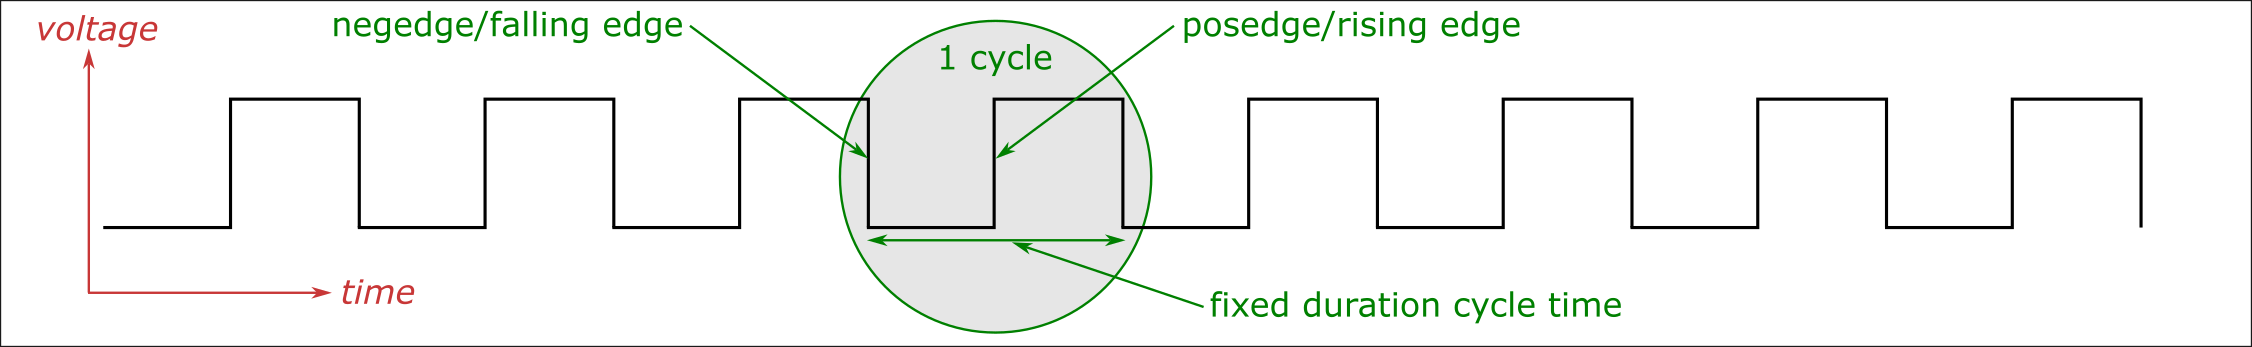
\includegraphics[width=6in,angle=0]{Figures/Fig_Clock}}
  \caption{\label{Fig_Clock} A clock signal}
\end{figure}
A clock signal is an electrical signal (a voltage on a wire), where
the voltage-change over time has the shape of a so-called ``square
wave'', which repeats, or ``cycles'', at a fixed time interval (the
``cycle time''), indefinitely.  Each cycle has a falling edge (or
negedge) and a rising edge (or posedge).  Modern FPGAs typically run
from 10s to 100s of MHz (``megahertz'', of millions of cycles per
second), and modern ASICs can run at up to several GHz (``gigahertz'',
or billions of cycles per second.  Thus, a clock is a real-time
reference signal.

Standard digital state elements ({\eg} registers) update their values
only and exactly on a clock edge (posedge or negedge), and hold that
value for the full next cycle, when they may change again.  Usually
all elements in a circuit react to the same edge, either the posedge
or the negedge; for simplicity we'll assume the posedge.

Specifically, if a D flip flop's EN input is high (1, true) at the
posedge, it updates its state to contain the value on the D input; if
the EN input is low (0, false), it does nothing, retaining its
previous value.  The value in the flip flop is continuously driven on
its Q output.

% ================================================================

\subsection{Constraints on mapping rules to a clock}

\label{Sec_Constraints_on_Mapping_Rules_to_a_Clock}

To map the collection of rules in a BSV design to clocked digital
hardware, as a first approximation, suppose that each rule was mapped
as suggested in Figure~\ref{Fig_Rule_Actions_1_2}.  Then,
conceptually, at each posedge, all enabled rules (whose CAN\_FIRE is
true) will fire and perform their output actions.

But this would be wrong, for two reasons:

\begin{itemize}

 \item \emph{Action Conflicts} or {\emph Resource Conflicts}: Two
       different rules may invoke the same action/actionvalue method
       (try to write the same register, or enqueue onto the same FIFO,
       dequeue the same FIFO, {\etc}.  As discussed in
       Section~\ref{Sec_Parallel_Conflict}, this is clearly not
       feasible at the same instant (same posedge).

 \item \emph{Ordering Conflicts}: The \emph{ordering} can be
       inconsistent with rule semantics.  Consider the execution of
       these two rules:

       \begin{center}
       \begin{minipage}{2.5in}
        {\small
        \begin{Verbatim}[frame=single, label=BSV]
rule rl_r1 (...);
   x <= y + 1;
endrule
        \end{Verbatim}
        }
       \end{minipage}
       \hmm
       \begin{minipage}{2.5in}
        {\small
        \begin{Verbatim}[frame=single,label=BSV]
rule rl_r2 (...);
   y <= x + 2;
endrule
        \end{Verbatim}
        }
       \end{minipage}
       \end{center}

       According to the one-rule-at-a-time semantics, either rule
       \verb|rl_r1| precedes \verb|rl_r2| or \emph{vice versa}.  In
       either case, register state-update by one rule is observed by
       the other rule.  Whereas, if we execute the rule actions at the
       same instant, neither rule observes the update by the other
       rule.  Thus, sequential execution and parallel, instantaneous
       execution will produce inconsistent results. (See also the
       Exercise at the end of
       Section~\ref{Sec_HW_representation_of_a_rule}.)

\end{itemize}

Recall in Figure~\ref{Fig_Rule_Actions_1} that a rule's CAN\_FIRE
signal controls its execution completely---if it is false, the rule
does nothing.  We take advantage of this observation in
Figure~\ref{Fig_Rule_Actions_Controlled}, where we pass the CAN\_FIRE
values of all rules through a \emph{Rule Controller} function which
returns, for each CAN\_FIRE, a corresponding WILL\_FIRE value.
\begin{figure}[htbp]
  \centerline{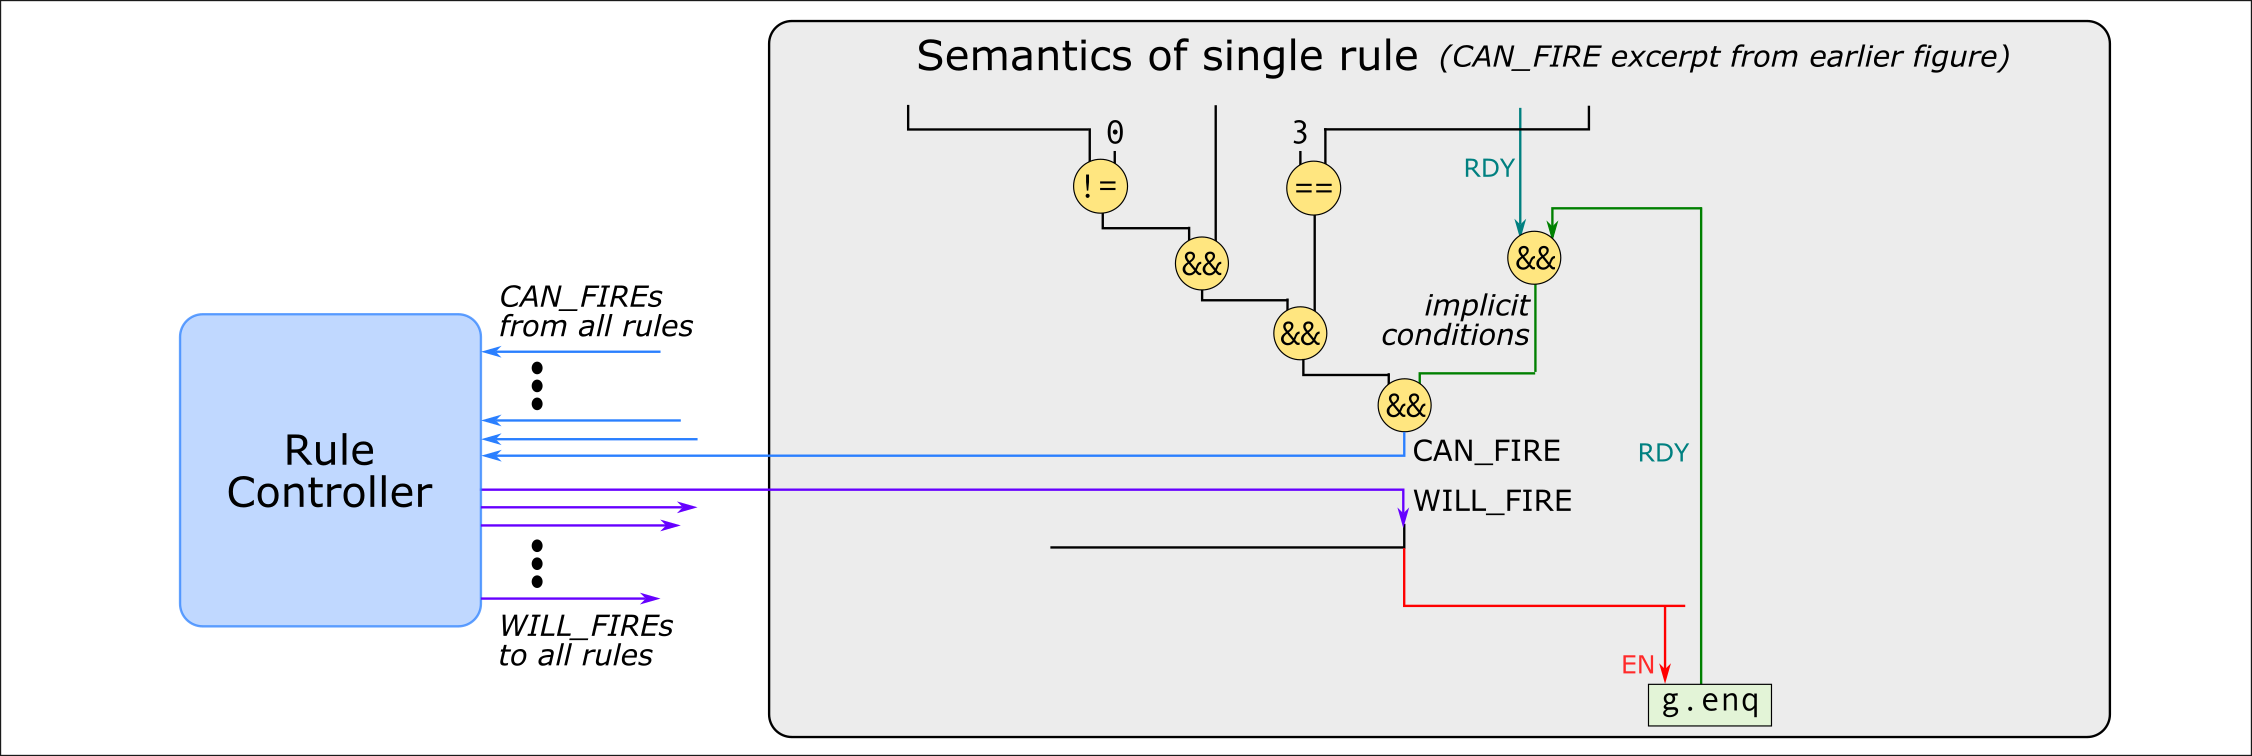
\includegraphics[width=6in,angle=0]{Figures/Fig_Rule_Actions_Controlled}}
  \caption{\label{Fig_Rule_Actions_Controlled}
           Controlling rule execution
	   (CAN\_FIRE excerpt from Figure~\ref{Fig_Rule_Actions_1_2})}
\end{figure}

Whenever a pair of rules \verb|rl_r1| and \verb|rl_r2| would conflict
if executed simultaneously, the Rule Controller ensures that it never
happens---if both CAN\_FIREs are true, the Rule Controller forces one
of the WILL\_FIREs to be false, {\ie} it suppresses one of the two
rules.

% ================================================================

\subsection{The Rule Controller produced by the \emph{bsc} compiler,
and reasoning about performance}

The abstract description of the Rule Controller above allows for many
possible implementations of the Rule Controller; the only criterion
for correctness is that the resulting rule execution in hardware
should be consistent with one-rule-at-a-time semantics.

The \emph{bsc} compiler produces a simple, state-free, combinational
circuit for the Rule Controller.  First, it produces a \emph{linear}
ordering of all the rules in the program, that results in minimal
conflicts (for example, if rule $rl_1$ reads a register and rule
$rl_2$ writes the same register, then it tries to place $rl_1$ earlier
than $rl_2$ in the ordering, because executing the rules
simultaneously would be consistent with that order, {\ie} would not
conflict.

Second, for any rule $rl_1$ before rule $rl_2$ in the ordering and
which would conflict if executed simultaneously, the WILL\_FIRE of
$rl_1$ is negated and AND-ed with the CAN\_FIRE of $rl_2$ to suppress
the latter rule.

A compile-time flag to the \emph{bsc} compiler will make it dump the
``schedule'', {\ie} the linear ordering of rules and the conditions
under which one rule may suppress another.

With this information, we can reason about the real-time perfomance of
a BSV program, {\ie} to address the question: ``does the program
compute something within the number of clocks we expect it to be
computed?''  Note, our unit of time is clock cycles, not real-time
\emph{per se} (seconds), because BSV has no way to know the actual
speed (1 MHz?  1 GHz?) of the clock you might supply to your hardware
circuit.

% ================================================================

\subsection{Explicit control of rule ordering, and controller optimizations}

We mentioned in the previous section that the \emph{bsc} compiler
produces a linear ordering of all the rules in a program, attempting
to minimize the number of conflicts.  This is a heuristic, because
producing an ``optimal'' ordering is undecidable.  Further, when the
compiler sees a conflict between two rules, it may have no criterion
to choose which one has priority, {\ie} which one will suppress the
other.  In such situations, the BSV programmer can provide explicit
\emph{attributes} on rules to guide the compiler's choice.

For example:

{\small
\begin{Verbatim}[frame=single,label=BSV]
rule rl_r1 (...);
   ...
endrule

(* descending_urgency = "rl_r1, rl_r2" *)
rule rl_r2 (...);
   ...
endrule
\end{Verbatim}
}

Here, the \verb|descending_urgency| attributes advises the compiler to
treat rule \verb|rl_r1| with higher priority.  The attribute is
written just before a rule; it can name this rule and any rules
earlier in the source text.

Another attribute advises the compiler, when there is no conflict, to
force \verb|rl_r1| to suppress \verb|rl_r2|:

{\small
\begin{Verbatim}[frame=single,label=BSV]
(* preempts = "rl_r1, rl_r2" *)
\end{Verbatim}
}

A third attribute asserts to the compiler that the CAN\_FIRE of two
rules are mutually exclusive, {\ie} can never simultaneously be true
(the compiler tries to prove such properties by itself, but cannot
always do so), which permits the compiler to simplify the controller.

{\small
\begin{Verbatim}[frame=single,label=BSV]
(* mutually_exclusive = "rl_r1, rl_r2" *)
\end{Verbatim}
}

In this case, the compiler also generates code that checks the
mutual-exclusivity property during simulation.

% ****************************************************************
